\documentclass[10.5pt,a4paper]{article}
\usepackage[a4paper,margin=2.2cm,top=2.3cm,bottom=2.4cm]{geometry}
\usepackage{fontspec}
\usepackage{unicode-math}
\setmainfont{TeX Gyre Pagella}
\setsansfont{Inter}[Scale=0.88]
\setmonofont{DejaVu Sans Mono}[Scale=0.80]
\setmathfont{DejaVu Math TeX Gyre}[Scale=0.95]
\usepackage{microtype}
\usepackage{xcolor}
\definecolor{accent}{HTML}{1F4E79}
\definecolor{muted}{HTML}{5F6670}
\definecolor{codebg}{HTML}{F6F7F9}
\definecolor{rule}{HTML}{D9DCE1}
\usepackage{graphicx}
\usepackage{booktabs,tabularx,array}
\usepackage{enumitem}
\setlist{nosep,leftmargin=1.4em,topsep=3pt}
\usepackage[font=small,labelfont={bf,sf},labelsep=period,skip=4pt]{caption}
\usepackage{titlesec}
\titleformat{\section}{\sffamily\large\bfseries\color{accent}}{\thesection}{0.7em}{}
\titleformat{\subsection}{\sffamily\normalsize\bfseries}{\thesubsection}{0.6em}{}
\titleformat{\subsubsection}[runin]{\sffamily\small\bfseries}{}{0em}{}[.]
\titlespacing*{\section}{0pt}{14pt}{6pt}
\titlespacing*{\subsection}{0pt}{10pt}{4pt}
\usepackage{fancyhdr}
\pagestyle{fancy}\fancyhf{}
\renewcommand{\headrulewidth}{0.4pt}
\renewcommand{\headrule}{\hbox to\headwidth{\color{rule}\leaders\hrule height \headrulewidth\hfill}}
\fancyhead[L]{\sffamily\footnotesize\color{muted}\ReportShortTitle}
\fancyhead[R]{\sffamily\footnotesize\color{muted}S. K. Eshraghi Naeini}
\fancyfoot[C]{\sffamily\footnotesize\color{muted}\thepage}
\usepackage{listings}
\lstset{language=C++,basicstyle=\ttfamily\footnotesize,keywordstyle=\color{accent}\bfseries,
  commentstyle=\color{muted}\itshape,stringstyle=\color{teal!70!black},numbers=left,numberstyle=\tiny\color{muted},
  numbersep=6pt,backgroundcolor=\color{codebg},frame=single,rulecolor=\color{rule},framesep=4pt,
  xleftmargin=14pt,breaklines=true,columns=fullflexible,keepspaces=true,showstringspaces=false,
  tabsize=4,aboveskip=6pt,belowskip=6pt}
\usepackage{tikz}
\usetikzlibrary{arrows.meta,positioning,shapes.geometric,calc,fit,automata}
\tikzset{blk/.style={draw=accent,thick,fill=accent!6,rounded corners=2pt,minimum height=8mm,minimum width=20mm,align=center,font=\sffamily\small},
         io/.style={font=\sffamily\footnotesize,align=center},
         arr/.style={-{Stealth[length=2mm]},semithick},
         st/.style={state,draw=accent,thick,fill=accent!6,minimum size=9mm,font=\sffamily\footnotesize,inner sep=1pt,align=center}}
\usepackage{xurl}
\usepackage[colorlinks=true,linkcolor=accent,urlcolor=accent,citecolor=accent]{hyperref}
\usepackage{siunitx}
\sisetup{group-separator={,},group-minimum-digits=4}
\newcommand{\sig}[1]{\texttt{#1}}
\newcommand{\pass}{\textcolor{green!45!black}{\textsf{\textbf{PASS}}}}
\newcommand{\fail}{\textcolor{red!70!black}{\textsf{\textbf{FAIL}}}}
\newcommand{\prt}{\textcolor{orange!80!black}{\textsf{\textbf{PARTIAL}}}}
\newcommand{\sev}[1]{\textsf{\footnotesize\textbf{[#1]}}}
\newcommand{\repo}{https://github.com/seyedkiarash/seyedkiarash.github.io/tree/main/projects/oop-circuit-simulator}
\newcommand{\note}[1]{\par\smallskip\noindent\colorbox{accent!7}{\parbox{\dimexpr\linewidth-2\fboxsep}{\small #1}}\par\smallskip}
\setlength{\parindent}{0pt}
\setlength{\parskip}{4pt}

\newcommand{\ReportTitle}[3]{%
  \thispagestyle{plain}
  {\sffamily\small\color{muted}Object-Oriented Programming \textbullet\ Department of Electrical Engineering, Sharif University of Technology\par}
  \vspace{2pt}
  {\sffamily\LARGE\bfseries #1\par}
  \vspace{1pt}
  {\sffamily\Large #2\par}
  \vspace{6pt}
  {\color{rule}\hrule height 0.6pt}
  \vspace{5pt}
  {\small
  \begin{tabular}{@{}l@{\hspace{2em}}l@{}}
    \textcolor{muted}{Student}  & Seyed Kiarash Eshraghi Naeini (403101383), team of two\\
    \textcolor{muted}{Instructor} & Dr.\ Abdollah Arasteh\\
    \textcolor{muted}{Semester} & Spring 2025 (second semester 1403--04) \quad\textcolor{muted}{review written:} #3\\
    \textcolor{muted}{Stack} & C++17/20, Eigen 3.4 (MNA solver), Qt 6 Widgets + Charts + Network, cereal (serialization)
  \end{tabular}\par}
  \vspace{4pt}
  {\color{rule}\hrule height 0.6pt}
  \vspace{8pt}}

\newcommand{\ReportShortTitle}{OOP course project -- circuit simulator code review}
\begin{document}
\ReportTitle{Circuit Simulator in C++}{Code Review of the OOP Course Project (Phases 0--2)}{October 2026}

\section*{Summary}
The course project was a SPICE-like circuit simulator built in three phases: an object-oriented design
(Phase~0), a command-line simulator based on modified nodal analysis (Phase~1) and a graphical
version with schematic entry, waveform viewer, project files and networking (Phase~2). It was a
two-person group project. This document reviews the \emph{final} code of each phase as it was
submitted; nothing was fixed or completed for this review. Both programs were rebuilt from source and exercised:
the Phase~1 simulator with scripted test circuits, cross-checked against \texttt{ngspice}, and the Phase~2
application under a virtual display with its analysis engine also tested on its own.

In short, the Phase~1 linear solver is correct where it is complete. Resistors, sources, the four
dependent sources it supports and backward-Euler transients of $RC$, $RL$ and $RLC$ circuits agree
with \texttt{ngspice} to the expected first-order accuracy. Several features are only partly working:
current-controlled voltage sources, inductors in DC analysis, ideal diodes and the ground command
(Section~\ref{sec:p1find}). The Phase~2 application has a clean MVC layout and a capable plotter,
but in the final version the schematic, the solver and the plot window are not connected end to end
(Section~\ref{sec:p2find}). Final code: \url{\repo}.

\section{Project timeline and scope}
\begin{table}[h]
\centering\small
\caption{Phases, deliverables and the code reviewed.}\label{tab:phases}
\begin{tabularx}{\linewidth}{@{}l>{\raggedright\arraybackslash}Xl@{}}
\toprule
Phase & Deliverable & Final code reviewed \\
\midrule
0 & Object-oriented design: classes, UML, design patterns, numerical methods, exception design (individual report) & design document, Apr 2025 \\
1 & Console simulator: LTspice-style commands, MNA with Eigen, transient and DC-sweep analysis, file menu & 1\,430 lines, one file, 10 Jun 2025 \\
2 & Graphical simulator: schematic editor, waveform viewer with cursors and math, AC/phase sweeps, sub-circuits, serialization, TCP networking & \num{5401} lines in 48 files, 4 Sep 2025 \\
\bottomrule
\end{tabularx}
\end{table}
The Phase~2 handout suggested SDL for the user interface; the team used Qt~6 instead (widgets,
\texttt{QGraphicsView} for the schematic, Qt Charts for plots and \texttt{QTcpSocket} for networking).
Where several copies of the code existed (backup folders, an archive and three GitHub repositories),
the file modification dates were compared and the newest complete copy was taken as final. For Phase~1
that is the working copy of the team repository, which is newer than its last commit. For Phase~2 it
is the \texttt{backup} folder, last edited on 4 September 2025.

\section{Phase 0 -- design intent}
The design report proposed a \texttt{Node} class, an abstract \texttt{Element} base with one derived
class per component, and a \texttt{Circuit} class owning both. It also proposed five patterns and techniques:
\begin{itemize}
  \item a \emph{Factory Method} for creating elements from parsed commands;
  \item a \emph{Bridge} between the circuit and interchangeable linear solvers (Gaussian elimination, LU or a library such as Eigen);
  \item \emph{MVC} for separating analysis from presentation;
  \item the \emph{Command} pattern for the console interface;
  \item an exception hierarchy (\texttt{SpiceException} with parsing, circuit and analysis subclasses).
\end{itemize}
Table~\ref{tab:design} at the end compares this plan with what was built.

\section{Phase 1 -- console simulator}

\subsection{Architecture}
The program is one translation unit organised in three marked sections, \emph{Models},
\emph{Controller} and \emph{View} (Fig.~\ref{fig:p1arch}). Elements derive from an abstract
\texttt{Element} that holds two \texttt{Node*} and exposes virtual getters. \texttt{MakingMNA}
assembles the MNA system and \texttt{MNASolver} solves it with Eigen's partial-pivot LU.
\texttt{TransientAnalysis} and \texttt{DCSweepAnalysis} drive the solver over time or over a source value. The
\texttt{centralController} owns nodes and elements and implements every command, and
\texttt{CommandParser} maps input lines to controller calls with one regular expression per command.

\begin{figure}[h]
\centering
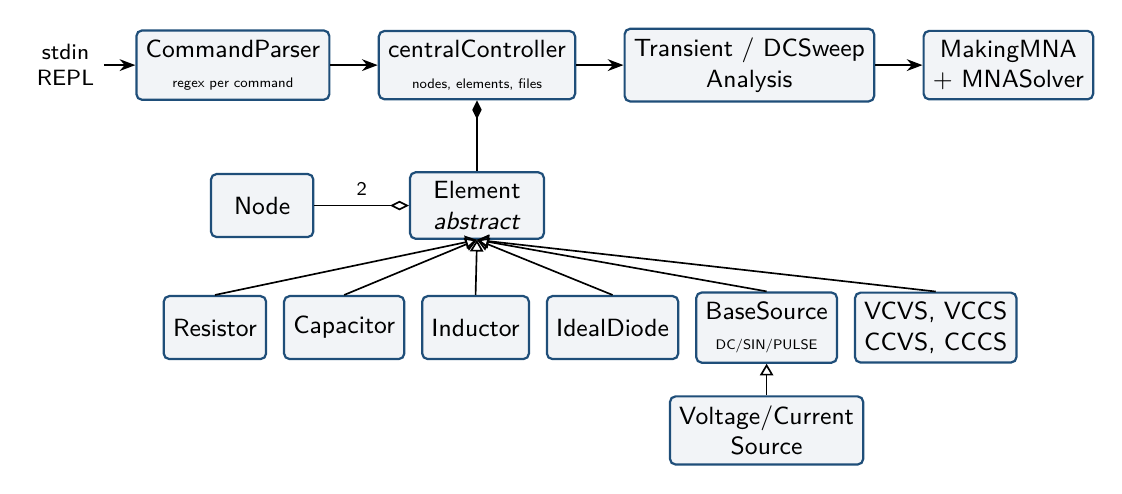
\begin{tikzpicture}[node distance=4mm and 5mm, every node/.style={font=\sffamily\scriptsize}]
\node[blk,minimum width=17mm] (el) {Element\\\textit{abstract}};
\node[blk,minimum width=13mm,below left=7mm and 18mm of el] (r) {Resistor};
\node[blk,minimum width=13mm,right=2mm of r] (c) {Capacitor};
\node[blk,minimum width=13mm,right=2mm of c] (l) {Inductor};
\node[blk,minimum width=13mm,right=2mm of l] (d) {IdealDiode};
\node[blk,minimum width=13mm,right=2mm of d] (bs) {BaseSource\\{\tiny DC/SIN/PULSE}};
\node[blk,minimum width=13mm,right=2mm of bs] (dep) {VCVS, VCCS\\CCVS, CCCS};
\node[blk,minimum width=13mm,below=4mm of bs] (vi) {Voltage/Current\\Source};
\foreach \x in {r,c,l,d,bs,dep} \draw[-{Triangle[open]},semithick] (\x.north) -- (el.south);
\draw[-{Triangle[open]},semithick] (vi) -- (bs);
\node[blk,minimum width=13mm,left=12mm of el] (node) {Node};
\draw[{Diamond[open]}-,semithick] (el.west) -- node[above]{2} (node.east);
\node[blk,above=9mm of el,minimum width=24mm] (ctl) {centralController\\{\tiny nodes, elements, files}};
\node[blk,left=6mm of ctl] (cp) {CommandParser\\{\tiny regex per command}};
\node[blk,right=6mm of ctl] (an) {Transient / DCSweep\\Analysis};
\node[blk,right=6mm of an] (mna) {MakingMNA\\+ MNASolver};
\draw[arr] (cp) -- (ctl); \draw[{Diamond[]}-,semithick] (ctl.south) -- (el.north);
\draw[arr] (ctl) -- (an); \draw[arr] (an) -- (mna);
\node[io,left=4mm of cp] (in) {stdin\\REPL};
\draw[arr] (in) -- (cp);
\end{tikzpicture}
\caption{Phase 1 class structure (inheritance: open arrows; ownership: diamonds).}\label{fig:p1arch}
\end{figure}

\subsection{Numerical method}
With $n$ non-ground nodes, the unknown vector holds the node voltages followed by one branch current
for each voltage source, inductor, diode, VCVS and CCVS. Each element adds (``stamps'') a few entries into
$A\,x = z$. Capacitors and inductors use the backward-Euler companion models
\begin{equation*}
  i_C^{k+1} = \frac{C}{h}\bigl(v^{k+1}-v^{k}\bigr), \qquad
  v_L^{k+1} - \frac{L}{h}\, i_L^{k+1} = -\frac{L}{h}\, i_L^{k},
\end{equation*}
so a capacitor is a conductance $C/h$ in parallel with a current source $C v^k/h$, and an inductor is an
extra row with $-L/h$ on the diagonal. The matrix is rebuilt and factorised at every time step. The
signs follow SPICE conventions: a source current is positive when it flows into the positive terminal, and VCCS
and CCCS currents flow from $n_+$ to $n_-$ through the source.

\subsection{Command interface}
Supported commands are listed below. Values accept SPICE suffixes (\texttt{k}, \texttt{meg}, \texttt{m},
\texttt{u}, \texttt{n}, \texttt{p}) and scientific notation.
\begin{itemize}
  \item \texttt{add R|C|L|D|V|I|E|G|H|F \dots}: add an element. Sources take a DC value,
    \texttt{SIN(off amp f)} or SPICE-style \texttt{PULSE(v1 v2 td tr tf pw per)}.
  \item \texttt{delete \textit{name}}: remove an element. Deletion is refused if the element is a
    control branch of a dependent source, and unused nodes are cleaned up.
  \item \texttt{nodes}, \texttt{list [type]} and \texttt{rename node \textit{old new}}.
  \item \texttt{.TRAN} and \texttt{.DC} define an analysis; \texttt{print TRAN|DC \dots\ V(\textit{n}) I(\textit{e})} runs it.
  \item \texttt{show existing schematics}, \texttt{NewFile \textit{name}}, a number to load a schematic, and \texttt{return}.
\end{itemize}

\subsection{Verification}
The final source compiles without warnings (\texttt{g++ -std=c++17 -Wall -Wextra}). Results were compared
with closed-form solutions and with \texttt{ngspice}-42 (Table~\ref{tab:p1tests}).

\begin{table}[h]
\centering\small
\caption{Phase 1 test circuits.}\label{tab:p1tests}
\begin{tabularx}{\linewidth}{@{}>{\raggedright\arraybackslash}Xl>{\raggedright\arraybackslash}X@{}}
\toprule
Test & Result & Observation \\
\midrule
Divider, DC sweep $0\to5$\,V; $V$, $I(R)$, $I(V)$ & \pass & exact; source current has SPICE sign \\
VCVS, VCCS, CCCS with resistive loads & \pass & identical to ngspice ($3$, $-1$, $2$\,V; $-1$\,mA) \\
$RC$ step, $h=\tau/10 \dots \tau/500$ & \pass & first-order convergence (Fig.~\ref{fig:order}) \\
Series $RLC$ step, $\zeta=0.16$ & \pass & matches ngspice (Fig.~\ref{fig:rlc}) \\
$RL$ step, inductor current & \pass & backward-Euler values \\
Input validation (negative/zero values, duplicate names, lower-case prefixes) & \pass & rejected with an error message \\
CCVS with grounded output terminal & \fail & exception \texttt{map::at} \\
CCVS with floating output & \fail & ``singular matrix'' \\
Inductor in DC sweep & \fail & ``singular matrix'' \\
Diode forward-biased by 5\,V & \fail & output stays 0\,V \\
\texttt{add GND b} on a circuit without a node named 0/GND & \fail & ``ground not detected'' \\
Four-resistor ladder, $R = 100$\,k$\Omega$ & \fail & false ``singular matrix'' (1 and 10\,k$\Omega$ pass) \\
Values \texttt{10uF}, \texttt{5mH}; \texttt{SIN(1, 2.5, 50)} & \fail & rejected (unit letter, commas) \\
Save and reload: \texttt{4.7n} capacitor; SIN source & \fail & saved as \texttt{0.000000}; SIN saved as DC \\
\bottomrule
\end{tabularx}
\end{table}

\begin{figure}[h]
\centering
\begin{minipage}{0.62\linewidth}\centering
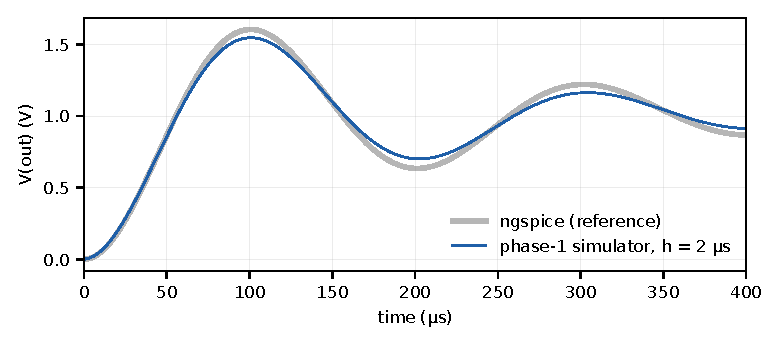
\includegraphics[width=\linewidth]{figures/rlc.pdf}
\caption{Series $RLC$ step response ($R=10\,\Omega$, $L=1$\,mH, $C=1\,\mu$F).}\label{fig:rlc}
\end{minipage}\hfill
\begin{minipage}{0.36\linewidth}\centering
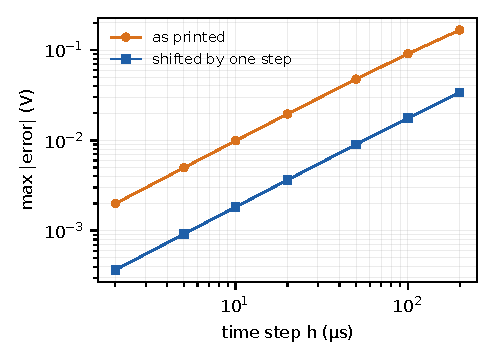
\includegraphics[width=\linewidth]{figures/order.pdf}
\caption{$RC$ step error versus time step.}\label{fig:order}
\end{minipage}
\end{figure}

The error falls linearly with $h$, as expected for backward Euler. The printed error, however, is
about five times larger than the method's own error. The reason is that the row labelled $t_k$
actually contains the solution at $t_{k+1}$: the loop solves first and then prints the old time.
Shifting the time column by one step leaves only the integration error (blue curve in Fig.~\ref{fig:order}).

\subsection{Findings}\label{sec:p1find}
Severity labels: \sev{H} wrong results or a crash, \sev{M} a missing or inaccurate feature, \sev{L} style or usability.
\begin{enumerate}[leftmargin=2em]
  \item \sev{H} \textbf{CCVS stamp is incomplete.} The CCVS row is written, but its branch current is never
    added to the KCL equations of its two nodes, so that column of $A$ is zero and the matrix is singular.
    For a grounded terminal the code also calls \texttt{nodeToIndexMap.at()} on the ground node, which
    is not in the map and throws.
  \item \sev{H} \textbf{Inductors in DC analysis.} In DC mode only the row $v_1-v_2=0$ is stamped. The current
    column is left out of KCL, so any circuit with an inductor fails the DC sweep.
  \item \sev{H} \textbf{Ideal diodes never conduct.} Diodes start \texttt{OFF} and nothing changes their state.
    An earlier commit (6 June) iterated the ON/OFF states at each step and also had an adaptive time step.
    Neither survived the merge into the final file.
  \item \sev{M} \textbf{\texttt{add GND \textit{node}} has no effect.} It only creates the node. Ground is recognised by
    name alone (\texttt{0}, \texttt{GND}, \texttt{gnd}).
  \item \sev{M} \textbf{Singularity test depends on scale.} A matrix is rejected when $|\det A|<10^{-12}$. The determinant
    shrinks as $G^n$, so ordinary high-impedance circuits are rejected. A rank or condition-number check on
    the LU factors would be scale-independent.
  \item \sev{M} \textbf{Saving loses information.} Values are written with \texttt{std::to\_string} (six decimals), so a
    4.7\,nF capacitor becomes \texttt{0.000000} and is dropped on reload, and 2.2\,$\mu$F becomes 2\,$\mu$F. SIN and
    PULSE sources are saved as their instantaneous value.
  \item \sev{M} \textbf{Units and syntax.} Suffixes followed by a unit (\texttt{uF}, \texttt{nF}, \texttt{mH}) are rejected.
    A bare \texttt{f} is read as farad, whereas SPICE reads it as femto. The dotted spellings in the
    handout (\texttt{.print}, \texttt{.nodes}, \texttt{.list}, \texttt{.rename}) are not accepted, and SIN arguments
    separated by commas fail, although the team's own test plan expected them to work.
  \item \sev{M} \textbf{Transient options.} Output is shifted by one step (see above). Initial conditions are all
    zero, with no DC operating point. The optional \texttt{Tstart} and \texttt{Tmaxstep} are parsed but ignored.
    \texttt{I(C)} always prints 0 because \texttt{Capacitor} does not override \texttt{getCurrent()}.
  \item \sev{L} \textbf{DC sweep side effect.} Sweeping a source calls \texttt{setValue()}, which permanently turns a
    SIN or PULSE source into a DC source.
  \item \sev{L} \textbf{Design.} Every analysis step uses long \texttt{dynamic\_cast} chains instead of a virtual
    \texttt{stamp()} on each element, so adding an element type means editing the matrix builder, the vector
    builder and the state update (not open for extension). Ownership is manual \texttt{new}/\texttt{delete}.
    Twenty-odd \texttt{std::regex} objects are compiled for every input line. The dense $O(n^3)$ factorisation is
    repeated each step although $A$ only changes when $h$ or a diode state changes.
\end{enumerate}
Strengths: the separation into model, controller and view is clear even within one file. Validation messages
follow the handout. Errors are thrown and caught at the REPL, so a bad command never ends the session.
Deletion protects control branches of dependent sources. Sign conventions agree with SPICE throughout.

\section{Phase 2 -- graphical simulator}

\subsection{Architecture}
The code is split into \texttt{Core}, \texttt{Model}, \texttt{Controller}, \texttt{View} and \texttt{Network}
folders (Fig.~\ref{fig:p2arch}).
\begin{itemize}
  \item \textbf{Model.} \texttt{Project} holds \texttt{shared\_ptr}s to elements and nodes plus the simulation
    settings, and is serialised polymorphically with cereal. \texttt{CircuitModel} translates a project
    into a new, struct-based \texttt{AnalysisEngine} (transient, AC and phase sweeps).
  \item \textbf{Controller.} \texttt{ApplicationController} saves and loads projects and sub-circuits and
    reports to the view through Qt signals.
  \item \textbf{View.} \texttt{GraphicsView} is the schematic editor, split into placement, wiring and
    editing files. Each component type has a \texttt{CircuitComponent} subclass that draws its symbol.
    \texttt{Plotter} reads result files in a worker thread and adds curves chunk by chunk.
\end{itemize}

\begin{figure}[h]
\centering
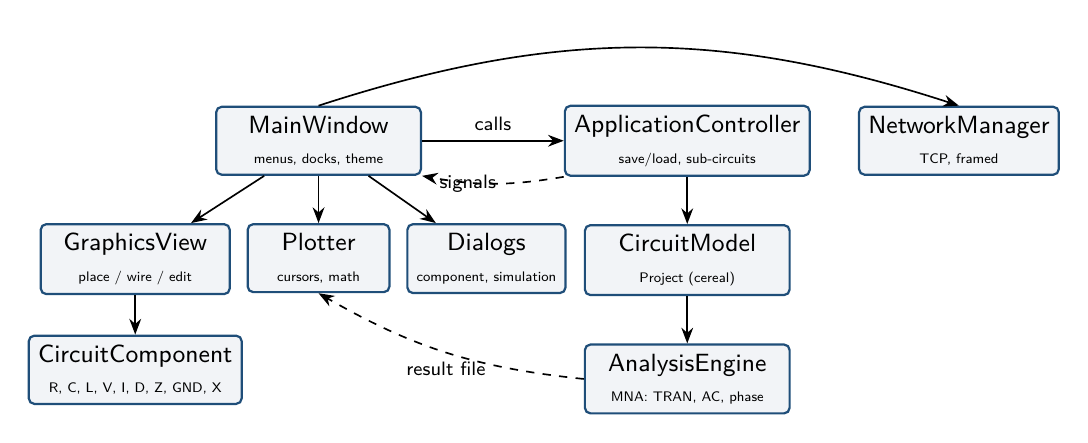
\begin{tikzpicture}[every node/.style={font=\sffamily\scriptsize}]
\node[blk,minimum width=26mm] (mw) {MainWindow\\{\tiny menus, docks, theme}};
\node[blk,below left=6mm and -2mm of mw,minimum width=24mm] (gv) {GraphicsView\\{\tiny place / wire / edit}};
\node[blk,below=6mm of mw,minimum width=18mm] (pl) {Plotter\\{\tiny cursors, math}};
\node[blk,below right=6mm and -2mm of mw,minimum width=18mm] (dl) {Dialogs\\{\tiny component, simulation}};
\node[blk,below=5mm of gv,minimum width=24mm] (cc) {CircuitComponent\\{\tiny R, C, L, V, I, D, Z, GND, X}};
\draw[arr] (mw) -- (gv); \draw[arr] (mw) -- (pl); \draw[arr] (mw) -- (dl); \draw[arr] (gv) -- (cc);
\node[blk,right=18mm of mw,minimum width=26mm] (ac) {ApplicationController\\{\tiny save/load, sub-circuits}};
\node[blk,below=6mm of ac,minimum width=26mm] (cm) {CircuitModel\\{\tiny Project (cereal)}};
\node[blk,below=6mm of cm,minimum width=26mm] (ae) {AnalysisEngine\\{\tiny MNA: TRAN, AC, phase}};
\node[blk,right=6mm of ac,minimum width=18mm] (nm) {NetworkManager\\{\tiny TCP, framed}};
\draw[arr] (mw) -- node[above]{calls} (ac);
\draw[arr,dashed] (ac.south west) to[bend left=10] node[left,pos=.4]{signals} (mw.south east);
\draw[arr] (ac) -- (cm); \draw[arr] (cm) -- (ae);
\draw[arr] (mw.north) to[bend left=18] (nm.north);
\draw[arr,dashed] (ae.west) to[bend left=12] node[below]{result file} (pl.south);
\end{tikzpicture}
\caption{Phase 2 structure. The dashed result-file path existed in the 20 August version and is not
used by the final menu (finding~2).}\label{fig:p2arch}
\end{figure}

\subsection{Building and running}
The final sources build with CMake, Qt~6.4 and system Eigen and cereal. The one change needed was the
\texttt{QDataStream::Qt\_6\_7} constant in the network code, which requires Qt~6.7 or newer. The application
crashed when the first component was placed (finding~1). The screenshots below therefore come from a
test build in which three pointer members were initialised to \texttt{nullptr}. That change is not in
the published code.

\begin{figure}[h]
\centering
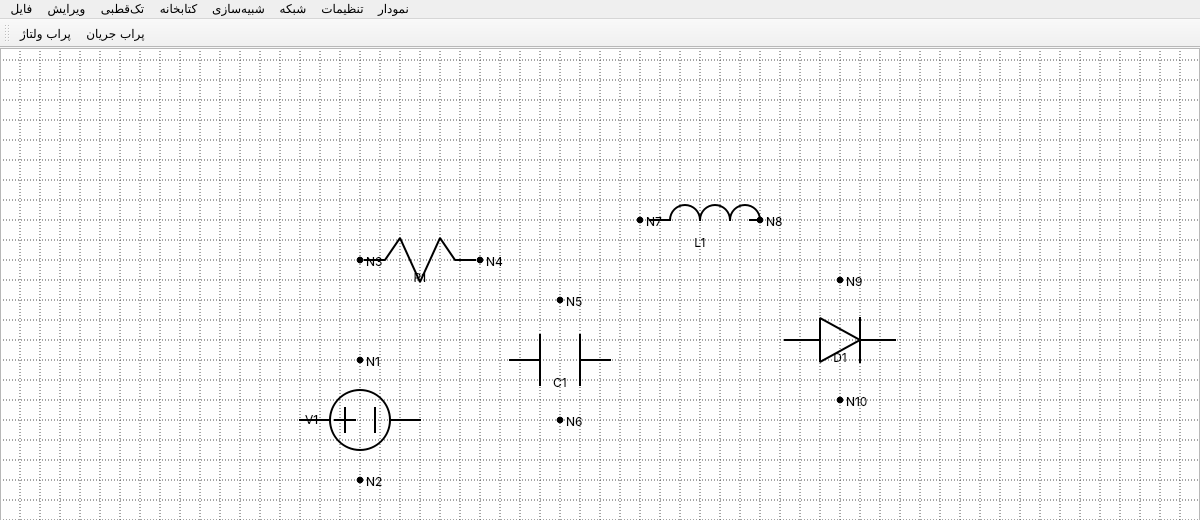
\includegraphics[width=0.9\linewidth]{figures/gui_place.png}
\caption{Schematic editor: a source, resistor, capacitor, inductor and diode placed with keyboard
shortcuts; the source, capacitor and diode were rotated by 90°. Each terminal gets its own node name
(N1, N2, \dots).}\label{fig:gui1}
\end{figure}

\begin{figure}[h]
\centering
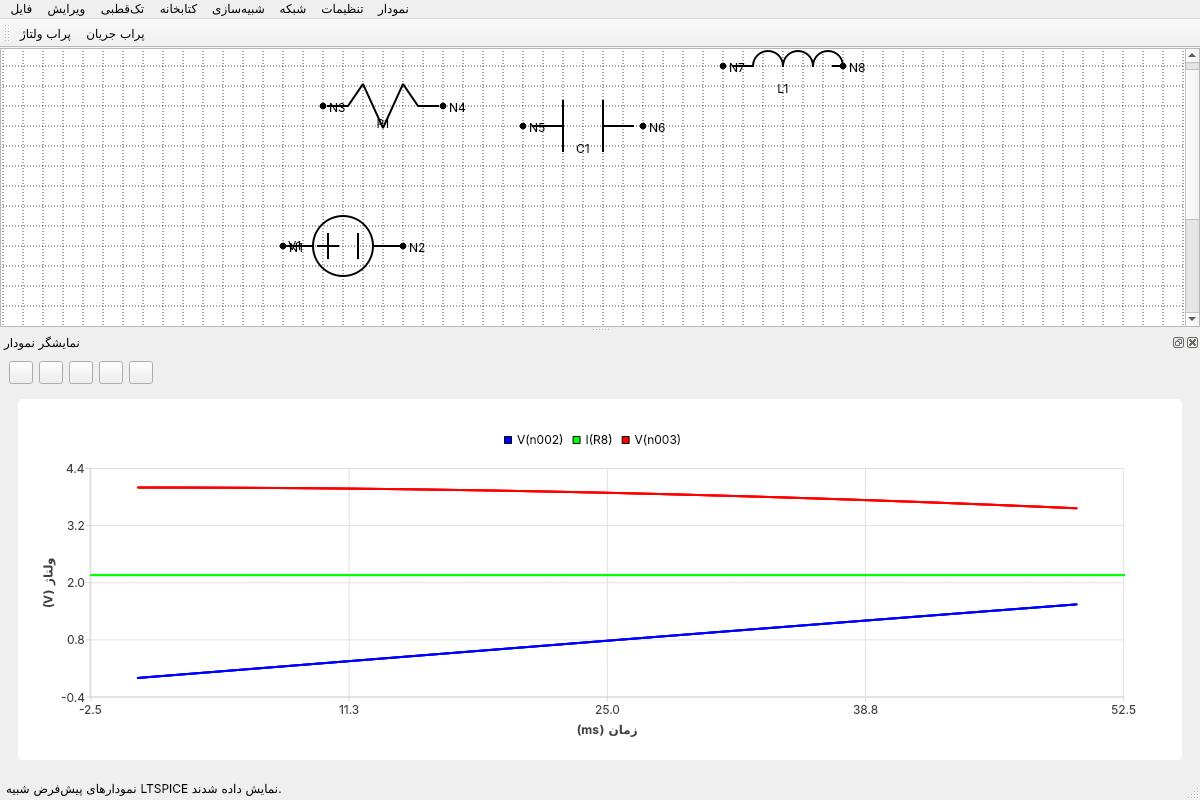
\includegraphics[width=0.9\linewidth]{figures/gui_charts.png}
\caption{After \emph{Simulation~$\rightarrow$ Settings and run} the waveform viewer shows three built-in
sample traces (labelled \texttt{V(n002)}, \texttt{I(R8)}, \texttt{V(n003)}), not results of the drawn circuit.}\label{fig:gui2}
\end{figure}

\subsection{Analysis engine}
Because the menu no longer calls the engine, it was tested directly with a small harness. The
transient solver uses the same backward-Euler models as Phase~1. For an $RC$ step with $h=\tau/100$, it
agrees with $1-e^{-t/\tau}$ to within 1\% of the step (largest error at $t=0$, from the same one-step offset). The AC solver builds a complex MNA system with admittances
$j\omega C$ and $1/(j\omega L)$, and its phasors are correct. However, the engine always reports the
\emph{first} non-ground node, which in a typical circuit is the source node (Fig.~\ref{fig:ac}). The
phase sweep is a stub: it runs the same AC point repeatedly without applying the phase, so its output
is constant.

\begin{figure}[h]
\centering
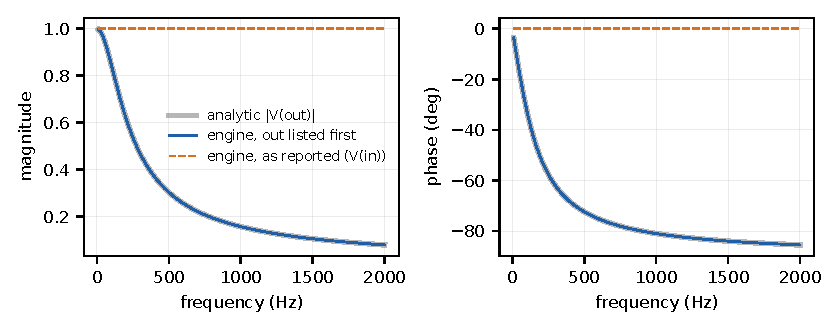
\includegraphics[width=0.86\linewidth]{figures/ac.pdf}
\caption{AC sweep of an $RC$ low-pass ($f_c=159$\,Hz). The solution is correct when the output node happens to be listed first (blue); as
written, the engine reports the source node, whose magnitude is 1 (orange).}\label{fig:ac}
\end{figure}

\subsection{Feature coverage}
Table~\ref{tab:cov} follows the course's scoring sheet. ``Partial'' means the code exists but the
feature does not work end to end in the final version.

\begin{table}[h]
\centering\small
\caption{Phase 2 requirements and their state in the final code.}\label{tab:cov}
\begin{tabularx}{\linewidth}{@{}>{\raggedright\arraybackslash}Xl>{\raggedright\arraybackslash}X@{}}
\toprule
Requirement & State & Note \\
\midrule
Graphical elements, shortcuts, grid snapping, rotation & \pass & R, C, L, V, I, D, Z, GND, sub-circuit symbols \\
Node labels and renaming; same-name nodes are joined & \pass & names are what connect a circuit \\
Wires connect elements without explicit nodes & \prt & wires are drawn but carry no connection \\
Transient analysis from the schematic & \prt & engine works; menu shows sample traces \\
AC sweep & \prt & first node only; linear sweep only \\
Phase sweep & \fail & stub \\
Probes (voltage/current/power) & \prt & cursor graphics only \\
Several signals, colours, rename, math ($+,-,\times,\div$) & \pass & math uses samples at matching times \\
Horizontal/vertical scaling, zoom, auto-zoom & \pass & menus and toolbar \\
Cursor and double cursor ($\Delta x$, $\Delta y$, slope) & \pass & \\
Sub-circuits: create, choose pins, save to library, reuse & \prt & stored and drawn, not simulated \\
Thevenin/Norton equivalent of a sub-circuit & \fail & not implemented \\
Waveform (sampled) source & \fail & a class exists but is not built or used \\
Project save/load with object serialization & \pass & cereal binary; round trip verified \\
Networking: send data, remote source, link two circuits & \prt & sends one element; no remote source \\
Name, icon, dark theme & \pass & \\
\bottomrule
\end{tabularx}
\end{table}

\subsection{Findings}\label{sec:p2find}
\begin{enumerate}[leftmargin=2em]
  \item \sev{H} \textbf{Uninitialised pointers.} \texttt{previewGraphics}, \texttt{previewWire} and \texttt{circuitModel} in
    \texttt{GraphicsView} have no initialiser. \texttt{startPlacing()} first calls \texttt{cancelPlacing()}, which
    deletes \texttt{previewGraphics} if it is non-null. With a garbage value this is undefined behaviour. On Linux it crashes
    (segmentation fault in \texttt{QGraphicsScene::removeItem}); on the team's Windows build heap memory was
    probably zeroed, which hid the bug.
  \item \sev{H} \textbf{The run command is disconnected.} \texttt{on\_actionRunAnalysis\_triggered()} now only calls
    \texttt{showDefaultCharts()}, which draws synthetic sine and DC traces. The 20 August version opened
    \texttt{SimulationDialog} and passed the settings to \texttt{ApplicationController::runAnalysis}, whose output
    file \texttt{Plotter} then loaded.
  \item \sev{H} \textbf{Connectivity by name only.} Each placed element and each wire segment gets new, uniquely
    named nodes, and the engine ignores \texttt{Wire} elements. Terminals therefore connect only when their
    nodes have the same name: ground symbols (all named \texttt{0}) or nodes renamed by the user. Merging
    coincident terminals and wire endpoints (e.g.\ with union--find) before building the netlist is the missing step.
  \item \sev{M} \textbf{Engine coverage.} Diodes, Zener diodes, sub-circuits and PULSE sources are skipped (PULSE
    evaluates to its DC value, 0). AC analysis drives every source, DC sources included, with its value. The
    octave/decade sweep option is ignored. Two fallback branches return made-up data (a constant magnitude of
    10, or the first source's voltage) instead of reporting an error. The dependent sources from Phase~1 were
    not carried over because the engine was rewritten instead of reused.
  \item \sev{M} \textbf{Serialization.} An earlier project file (\texttt{t1.proj}, 16 August) no longer loads
    (``failed to read 4 bytes''), most likely because the class layout changed and no cereal class versions are declared. Saving a sub-circuit copies the project's \texttt{shared\_ptr}s,
    so the definition aliases the live circuit until it is written to disk.
  \item \sev{M} \textbf{Networking.} Messages are length-prefixed (good), but the expected size is stored in a
    member shared by all client sockets. \texttt{waitForConnected} blocks the GUI thread for up to 3\,s, and
    \emph{Send data} transmits only the first element of the project.
  \item \sev{L} \textbf{View details.}
    \begin{itemize}
      \item Rotation moves the terminals but draws the body unrotated (Fig.~\ref{fig:gui1}).
      \item \texttt{ZenerDiodeView} is never created, because the \texttt{dynamic\_cast<Diode*>} test is reached first.
      \item The shortcuts \texttt{Ctrl+C}, \texttt{Ctrl+V} and \texttt{Ctrl+Z} override copy, paste and undo.
      \item Toolbar icons come from \texttt{QIcon::fromTheme}, which is empty on Windows, so the buttons are blank.
      \item In dark mode the symbols are drawn black on a dark background.
    \end{itemize}
  \item \sev{L} \textbf{Dead code.} Eleven root-level files are not in \texttt{CMakeLists.txt}: \texttt{waveformsource},
    \texttt{componentlibrary}, \texttt{nodelabel}, \texttt{subcircuitcomponent} and \texttt{wire} (header and source each),
    and \texttt{main2.cpp}, a copy of the Phase~1 program.
\end{enumerate}
Strengths: the folder-level MVC split is consistent, and the view talks to the controller only through
methods and Qt signals. Element ownership uses \texttt{shared\_ptr}, and cereal's polymorphic registration
gives one-line project save/load; a saved project (\texttt{t5.proj}) loads and round-trips correctly. The
plotter is the most complete part. It reads data in a background thread in chunks, as the handout
recommends for long simulations, and offers auto-zoom, independent axis scaling, colour and name
changes, math traces and single and double cursors.

\section{Design plan versus implementation}
\begin{table}[h]
\centering\small
\caption{Phase 0 proposals and how they appear in the code.}\label{tab:design}
\begin{tabularx}{\linewidth}{@{}l>{\raggedright\arraybackslash}X@{}}
\toprule
Proposal & Implementation \\
\midrule
Abstract \texttt{Element}, polymorphism & Used in both phases; behaviour is selected with \texttt{dynamic\_cast} rather than virtual methods \\
Factory Method for parsing & \texttt{CommandParser} plus one \texttt{making\dots()} method per element (Phase~1); \texttt{startPlacing()} maps type names to classes (Phase~2) \\
Bridge for linear solvers & Not used; Eigen \texttt{PartialPivLU} is called directly \\
MVC & Sections in Phase~1; folders, a controller and Qt signals in Phase~2 \\
Command pattern for the console & A regex dispatcher with direct calls, not command objects \\
\texttt{SpiceException} hierarchy & Standard \texttt{logic\_error}/\texttt{runtime\_error} with descriptive messages \\
Euler or Runge--Kutta integration & Backward Euler (implicit, stable for stiff $RC$ circuits); adaptive step tried, then dropped \\
\bottomrule
\end{tabularx}
\end{table}

\section{Lessons}
\begin{itemize}
  \item Give each element a virtual \texttt{stamp(A, z, h)} method. The solver then never needs to know element types, and
    Phase~2 could have reused the Phase~1 engine, dependent sources included.
  \item Build the netlist from geometry: merge terminals that touch and the endpoints of wires, then name the nets.
  \item Keep a small set of golden circuits with reference results (here from ngspice) and run them on every
    change. Most findings above are regressions that such tests catch immediately.
  \item Initialise every pointer member and build on a second platform; uninitialised members often work on one
    compiler and crash on another.
\end{itemize}

\section*{How this review was done}
Phase~1 was compiled with \texttt{g++}~13.3 and Eigen~3.4 and driven through standard input by scripts.
Reference results came from \texttt{ngspice}-42 and closed-form solutions. Phase~2 was built with CMake, Qt~6.4.2
and cereal, run under Xvfb with input from \texttt{xdotool}, and debugged with \texttt{gdb}. Its analysis engine
and serialization were tested with small C++ harnesses linked against the original source files. The published
code is the final submitted version, without third-party libraries and build folders: \url{\repo}.

\end{document}
